%% The basic red thread of this theoretical framework

%% Problems
% Problems UX designers have to consider (UX is defined elsewhere)
% Problems specific to mobile - no long sessions etc, small attention span, app stickiness etc
%% Usage
% Motivation - What drives the user to use a app?
% App discoverability - Mention the problem, but do not go into depth
% What are the kinds of behavior that can be used when using the application? (skill, rule, knowledge) - Segment into mental models
% Mental models - What are they and how do they work? How are they relevant to UX? How are they measured? - Segment into Gulf of evaluation and execution
% Gulf of evaluation and execution - Description and relevance
%% Bridging the gap
% Direct manipulation
% Learnability - Could be seen as adjusting the mental model in this context?
% Feedback and response through Human Computer Dialogue?
%% Design
% Cognitive load - How to design to reduce cognitive load
% Affordances / Signals
% Incidental learning
% Memory
% Language - Articulatory and Semantic distance

\chapter{Theoretical Framework}
\label{chap:theoretical_framework}
Designing and gathering material for a theoretical framework for user onboarding is a challenging tasks. The onboarding process covers a lot of different aspects of user experience design

\section{Literature study}
% Literature reviews are designed to provide an overview of sources you have explored while researching a particular topic and **to demonstrate to your readers how your research fits into the larger field of study**
\ignore{Make sure that we define when onboarding starts and stops.}
There hasn't been a lot of academic research in the field of user onboarding, even though there is a lot of research regarding employee and manager onboarding (ref) (ref) (ref). The most notable contributions to the research field of user onboarding is by Oechsner \cite{Oechsner2016}, where she presents general guidelines for onboarding a user to a digital platform. The guidelines she presents are supported by psychology and IxD research, but fail to include the body of work of employee onboarding and the marketing aspect \textit{stickiness}. Also, her guidelines are meant to be general and may not alone aid the entire onboarding process of all platforms. Her study of user onboarding has been exhaustive, but with the circumstances related to the different usage model of mobile applications support the need for revisiting onboarding process.

\subsection{Onboarding}
\ignore{Include more onboarding sources}
The definition and the steps required of onboarding varies across literature.

\section{Theoretical Background}
% User problems -> Mobile -> Value proposition
To better understand how to provide a good onboarding experience for the mobile app user we have to understand the problems associated with UX-design, both in general and problem mobile devices. We then structure the Theoretical Background with the subsections \textit{acquisition}, \textit{accommodation}, \textit{assimilation} and \textit{acceleration}. These concepts stems from business management context, but to explain them in a user-experience we draw inspiration from cognitive and behavioral psychology. Cognitive psychology is a branch of psychology which study higher mental processes of the human mind such as attention, language use, memory, perception, problem solving, and thinking \footnote{\url{http://www.apa.org/research/action/glossary.aspx?tab=3}}. Behavioral psychology and its research field is focused on the environmental determinants of learning and behavior. With the combined resources of these fields of research we define motivations of users to use an application. We briefly discuss the domain of application discoverability and and its relevancy to onboarding.

\subsection{Acquisition}
% Acqusition Få tag i och förstå sina användare. Hur gör man detta? Man definierar och designar för sin målgrupp, och förstår deras motivation och ge dem vad de behöver. Det finns metoder för detta så som att skapa Personas. Det finns även ett problem så som marknadsföring och app discoverability, men vi ska inte täcka det i denna rapport.
Acquisition is the act of identifying, recruiting, selecting and getting people to join \cite{Bradt2009}. To be able to get people to join, the designer has to make sure the app communicate its value proposition to the correct target market, make sure the app is discoverable to the user, motivate the user download and use the app.

\subsubsection{Target market}
% Identifying the market

\subsubsection{Needs}
% Identify the motivation of the user base, explain what motivation is.
To be able to understand how to provide a good user experience, we have to understand the needs of the user, and what value is important to the user to fulfil their need. Maslow’s theory of motivation \cite{Maslow1943} state that humans are motivated by a hierarchy of needs; The 'physiological', the safety, the love, the esteem need and finally the need of self-actualization. Physiological needs are the classic instances of hunger, sex and thirst. Serving one of needs may act as a channel for other needs; someone might be eating because they seek comport rather than for vitamins or nutrients. He explains that when one hierarchy of need has been satisfied the human try to satisfy the next need in the hierarchy, and that the subsequent need has to be fulfilled to be able to care for any of the other needs; "A person who is lacking food, safety, love, and esteem would most probably hunger for food more strongly than for anything else.". The need for safety is the act of seeking a stability in the world where we are away from dangers. If both the physiological and the safety needs are met, then the need for love and belongingness is at the center of concern. The person is now concerned with having friends, a partner and/or children, and will take great strides to do so. When the esteem needs emerge after we have satisfied the physiological, safety and love needs, we strive for a high evaluation of ourselfs, for self-respect, or self-esteem, and for the esteem of others. We want to be respected and valued by others, and this need may strive people to engage in a profession or hobby to gain recognition. Maslow states that this need can be divided into two sets. The first is the desire of self-respect, independence and freedom. Secondly we have the desire for respect from others. Finally, when all precedent needs have been satisfied we reach the need for self-actualization, which refers to the need of self-fulfillment. "What a man \textit{can} be, he \textit{must} be"

% Read Hazzenzahl 2010

\subsubsection{Motivation}

Motivation is what drives human to accomplish things, keeps them interested and committed \ignore{\cite{Ryan and Deci, 2000}}.

At the level of self-determination, we distinguish between different types of motivation; \textit{intrinsic} and \textit{extrinsic} motivation \cite{Ryan2000a}. These differ in the reason or goal that prompts the execution of some action. Intrinsic motivation specifically refers to the act of doing something due to it being interesting or enjoyable, and extrinsic motivation refers to the act o doing something because it leads to a favorable outcome.  The word \textit{Intrinsic} is defined as "belonging to a thing by its very nature"\footnote{\url{http://www.dictionary.com/browse/intrinsic}}, and intrinsic motivation is thought to be a fundamental aspect of the human creature \cite{White1959}. Since we were born, we've had a curiosity of the world with no external incentives to learn and explore it \cite{Ryan2000a}. Extrinsic motivation is the underlying reason an activity is performed to attain some outcome. The final outcome is the facilitator of the activity, and not the activity itself \cite{Ryan2000a}. This is also the main problem with extrinsic motivation; when the external factors dissappear so does the motivation \ignore{\cite{Hassenzahl2010}}. It is believed from operant theory that all behaviors are motivated by rewards \ignore{\cite{Skinner1953}}, therefore intrinsically motivated people perform a task because the task itself is rewarding to them, while extrinsically motivated people only perform it to achieve the external reward. Research suggest that higher levels of intrinsic motivation typically lead to a higher willingness to spend more time on a task \ignore{\cite{Deci1975} download from torrent}. Intrinsic motivation is regarded as the better of the two when designing user experiences, but may be harder for the designer to create.

To improve the users intrinsic motivation, the user interface designer can relate the content and objectives of the application to the needs and interests of the learner \ignore{\cite{Keller1983}}. This can be done by using familiar metaphors and analogies \ignore{\cite{Curtis1984}}. Instructions provided to the user that use a personal style (e.g personal pronouns, names of specific people) rather than formal style may stimulate the user to learn. Also, providing immediate, positive and informative feedback in a context may improve intrinsic motivation, but not neccessarily increase or decrease performance \ignore{\cite{(Bates, 1979; Condry, 1977; Deci, 1975, 1971; Keller, 1983)}}. Humor, on the the other hand, has been found to not improve motivation since it can distract the user and interfere with comprehension \ignore{\cite{Markiewicz, 1974; Sternthal & Craig, 1973}}.

Motivation will not alone prompt a user to perform a target behavior. The following sections will discuss a model developed for understanding user informational system adoptance and a behavioral model for persusasive design.

\subsubsection{Technology Acceptance Model}
While there are other theoretical models developed to explain user acceptance and usage behaviour of information technologies, the Technology Acceptance Model (TAM) \cite{Davis1989} \cite{Davis1989a} is the most widely accepted model and has been validated numerous times, e.g. \cite{Hu1999} \cite{Chau1996} \cite{Mathieson1991}. TAM explain the behavioral intention to use an technology with two major beliefs; \textit{perceived ease of use} and \textit{perceived usefulness}. Perceived ease of use is how much a person believes that the use of some technology will be free of effort. This is believed to be a process of expectancy, since the perceived ease of use is defined in terms of expected effort the user is able to report whether or not their expectancy is correct. Perceived usefulness is how much a person believes that using a technology will enhance their productivity. These two beliefs correlate with eachother, as perceived usefulness is an outcome of the users expectancy. A positive perceived ease of use will positively influence perceived usefulness, as when the technology is easier to use, the more useful it can be. Davis \cite{Davis1989} has found that perceived ease of use has a direct effect on intention, and in an indirect effect on intention via perceived usefulness, and that it is an initial hurdle for users to overcome for acceptance, adoption and usage of a system \cite{Davis1989a}. Figure \ref{fig:TAM} represent the theoretical model.

\begin{figure}[h]
  \centering
    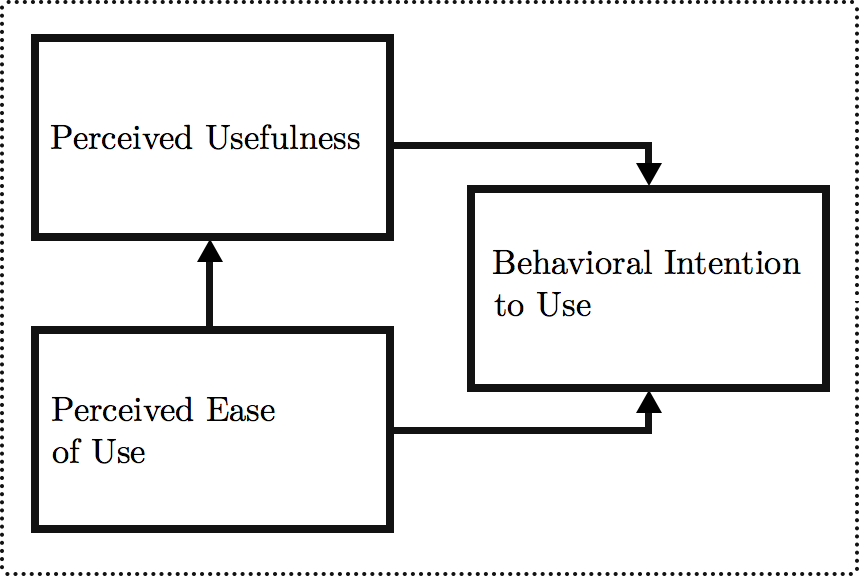
\includegraphics[width=0.6\textwidth]{TAM}
  \caption{Theoretical model of Technology Acceptance Model.}
  \label{fig:TAM}
\end{figure}

This model implicitly indicate that external variables influence perceived ease of use and perceived usefulness. There has been several studies which has defined some of these external variables and extended the model with constructs such as intrinsic motivation, control, emotion \cite{Venkatesh2000}, flow theory \cite{Koufaris2002} and trust \cite{Gefen2003}.

To design an interface to increase perceived ease of use there are a number of ways we can do this. Tractinsky et al. has found a strong correlation between aestethics and perceived usability, which remain intact from the users intial use to continued use \cite{Tractinsky2000}.

\ignore{
System designers typically attempt to build systems that are easy to use while providing the functionality that the users need to accomplish their tasks. While user interface design is the typical focal point to enhance user acceptance, this research shows that there are multiple factors not directly related to the user system interaction that are perhaps more important (e.g., computer self-efficacy). While a large amount of time during system design and development is typically spent on the user interface, this research suggests that practitioners should spend more time creating a favorable impact on system-independent factors, which have clearly been shown to be more important than user perceptions that relate to the user-system interaction in determining perceived ease of use of a specific system. This is particularly important since at all stages of user experience with a system, general, system-independent constructs play a stronger role than constructs that are a result of the user-system interaction.

Similarly, research should focus on designing managerial interventions that will provide facilitating conditions that favor the creation of positive perceptions about the ease of use of a specific system via perceptions of external control. Researchers and practitioners should attempt to better leverage the individual difference variable of computer playfulness and system-specific perceived enjoyment during the design and development phases of system building, and attempt to incorporate it into end-user training situations. In general, practitioners should design interventions directed at the various determinants of perceived ease of use that go beyond traditional training methods, which typically aim to impart only conceptual and procedural knowledge about a specific system. Organizations should consider putting in place general computer training programs that target increasing computer awareness, enhancing computer self-efficacy, and reducing computer anxiety among employees. Such training programs combined with appropriate facilitating conditions should pave the path for acceptance and usage of new systems. In fact, organizations will benefit particularly from system-specific training interventions that enhance user perceptions about the specific system and their general beliefs about new information technologies (see Compeau 1992).
One of the areas that has not been exploited in practice is the potential for intrinsic motivation to enhance user acceptance and usage. Much prior research (Davisetal.1992;Malone1981a,1981b;Websterand Martocchio 1992; Venkatesh and Speier 1999) has found intrinsic motivation to be an important factor influencing user acceptance and learning. This research has further refined our understanding in this regard by suggesting that general computer playfulness and perceived enjoyment are determinants of perceived ease of use. One example is “fun icons” like the ones introduced in MS-Office 97. A similar example is the use of “warm and fuzzy” screen savers (e.g., flashing cartoons on the screen, some action related to your favorite basketball team, etc.) as a way to cause perceived ease of use of specific systems (used by the individual) to be more favorable. Recent work in IS (Venkatesh 1999) and organizational behavior}

\subsubsection{Intention}
Motivation drives intention.

\subsubsection{Value}
% Intrinsic value and extrinsic value

\subsubsection{Discoverability}
App discoverability is the concern of finding the correct app. \ignore{Expand, a lot}

\subsection{Accommodation}
% Accommodation Ge användare de verktyg de behöver för att lyckas. Implicit innebär dessa verktygen att de är användarbara också. Mentala modeler osv. Designa för användning med context.
Accommodation is the act of giving the users the tools they need to be able to succeed \cite{Bradt2009}. For the users to efficiently use the tools given, we have to understand their behavior; how they reason and learn.

\subsubsection{Behavior}
\cite{Rasmussen1983} has identified three typical levels of performance. \textit{The skill-based behavior} represent the subconscious actions and activities which we perform on a "smooth, automated, and highly integrated patterns of behavior". This level of performance is based on a simple feedback loop, where a stimuli facilitate a motor output. \ignore{Provide example of this}

\textit{Rule-based behavior} are patterns of behavior which emerge from previous and similar actions performed in a previous similar occasion. The user acts in a goal-oriented manor where the user tries to achieve a goal, which is usually not explicitly stated, with the rules that has empirically evolved through previous successful experiences. \ignore{Find evidence that rule and skill-based behavior might help the user with cognitive load}

The main differences of skill-based and rule-based behavior is that the person may not consciously be aware of the actions the user perform when performing actions on a skill-based level, and may not be able to recollect why such an action has been taken. The higher level rule-based actions are generally based on "explicit know-how, and the rules used can be reported by the person".

The third, and final level of performance as \cite{Rasmussen1983} has identified, is \textit{knowledge-based}. Knowledge-based performance is used during situations that the user is not familiar with, and where any know-how or rules cannot be used from previous experiences. \cite{Rasmussen1983} states that "In this situation, the goal is explicitly formulated, based on an analysis of the environment and the overall aims of the person. Then a useful plan is developed-by selection-such that different plans are considered, and their effect tested against the goal, physically by trial and error, or conceptually by means of understand the functional properties of the environment and prediction of the effects of the plan is considered." At this level of abstraction, the user represent the system in an internal construct called \textit{mental model}.

\subsubsection{Mental model}
A common concept in the field of cognitive psychology is the concept of \textit{mental models}. Mental models was first introduced by American philosopher Charles Sanders Peirce, where he argues that humans reason by a process which
"...examines the state of things
asserted in the premises, forms a diagram of that state of things, perceives in the parts of that diagram relations not explicitly mentioned in the premises, satisfies itself by mental experiments upon the diagram that these relations would always subsist, or at least would do so in a certain proportion of cases, and concludes their necessary, or probable, truth." \cite{Pierce1974}

This was further elaborated by the psychologist Kenneth Craik, where he proposes that humans construct "small-scale models" of external reality \cite{Craik1967}. These mental models enable us to use past events to be able to react to present events and anticipate future events, to reason, and to understand our environment. Since Craik's contributions, cognitive psychologist has argued that mental models are formed through current and general knowledge, perception and imagination \cite{Johnson-Laird2001} \ignore{Find some more citations to support this claim}. In the field of Human-Computer Interaction (HCI) mental models has sometimes been used interchangeably with cognitive and conceptual models, and their difference and usage might be confusing as \cite{Staggers1993} concludes. For the purpose of this paper, we'll be using Normans \cite{Norman2013a} definition of conceptual and mental model, where he states that mental model needs to be consistent with the designers conceptual model. Mental models are the models made from experience, instruction and training which users interact through \cite{Norman2013a}, and the models become more mature as the user experience increase \cite{Barker1998}. Mental models of devices are created mostly through perceiving possible actions and its visible structures afforded by its interface \cite{Norman2013a}. The mental model of the user guide the users expectation of the application, and can guide the users navigation, planning of actions and contribute to the interpretation of interfaces feedback \cite{Jin1992}\ignore{not the actual source}. Mental models may act as both facilitators and inhibitors when learning, depending on the new information \cite{Cho1996}. When the user has acquired an adequate mental model of the structure and possible functions of the system the user is less likely to become disoriented \cite{Jih1992}, but if the user has trouble fitting new information into their current mental mode they experience frustration \cite{DApollonia2004}.

Norman \cite{Norman2013a} provide us with a seven-stage model which describe the manor by which users use interactive products.
\begin{enumerate}
  \item Forming the goal
  \item Forming the intention
  \item Specifying the action
  \item Executing the action
  \item Perceiving the system state
  \item Interpreting the system state
  \item Evaluating the outcome
\end{enumerate}

This model of actions help us describe how an user explore an interface \cite{}\ignore{Polson and Lewis, 1990}. This approximate model \cite{Norman2013a} is not consciously used by the user, but rather it tries to explain how we perform tasks. The model is cyclic, meaning that the user will experience multiple loops of the model as they explore an interface. The model is developed on the basis that human actions has two aspects; execution and evaluation. Execution is doing something which affect the world, and evaluation is the comparison if the world reached or got closer to a state which was desired by the user. These two aspects have their of stages of performance. The stages of execution involves forming the goal, which may be an abstract representation of what we want to achieve (get to work, eat dinner, pick a movie). The goal forms our intentions to perform an action, which constitutes in an action sequence to be executed to satisfy the intention. Finally in the stage of execution, the action sequence is executed upon the world and we reach the stages of evaluation. The first stage of evaluation is perceiving the systems state. The perception is then interpreted according to our expectations and finally compared to our intentions and goal. As the users try to finish their tasks, there are four critical points where user errors can occur, as identified by \cite{Shneiderman2004}:
\begin{enumerate*}
  \item users form an inadequate goal,
  \item users might not find the correct interface touchpoint because of a label or icon that does not sufficiently represent its corresponding action
  \item users may not know what action to perform to get a desired output and
  \item users get misleading feedback from the system
\end{enumerate*}

%%BRIDGING THE GAP

\subsubsection{Gulf of evaluation and execution}
% Expand this section.
The user initially start with an intention of achieving a goal, where the goal is often expressed in psychological terms. The system or interface

\subsubsection{Direct manipulation}

Direct manipulation was first introduced by Shneiderman, which describe a system which inherit the following properties (p. 184 erryday things as well):

\begin{enumerate}
  \item Continuous representation of the object of interest
  \item Physical actions or labeled button presses instead of complex syntax
  \item Rapid incremental reversible operations whose impact on the object of interest is immediately visible
\end{enumerate}

\subsubsection{Learnability}
More often than not, "interface usage requires learning" \cite{Grossman2009}. Even though there’s plentiful of research regarding learnability, its definition is not widely agreed upon. The different definitions consider different scopes of learnability, e.g. Nielsen definition consider the initial learning curve of the user, and that a highly learnable system would be "allowing users to reach a reasonable level of usage proficiency within a short time." What "a reasonably level of usage proficiency" is relative to a "short time" is still unclear, and it leaves a lot to our own imagination. Schneiderman et al. provide us with a more general applicable definition of "the time it takes members of the user community to learn how to use the commands relevant to a set of tasks". Schneiderman et al. also discuss a different aspect which tightly coupled with learnability, which is \textit{Retention over time}; How well is the user able to recall how to use an application after a specific time period? Retention may

\subsubsection{Feedback}
Feedback...

\subsubsection{Human-Computer Dialogue}

If the conceptual model is not clearly communicated to the user and is not properly corrected through computer-human dialog, the user will have trouble performing the tasks they've set out to solve their problem. Studies of blame \ignore{Find these studies}, or \textit{attribution}, has shown that when a fault occurs in a system, the person in question is more likely to attribute the error to system than their own. Similarly, when fortune occurs to a person they are likely to attribute the fortune to their person and intelligence.

If the users mental model is not consistent with the conceptual model provided by the designer, the users mental model can be modified through a \textit{computer-human dialog}

The communication between a user and a computer-based system is through a \textit{user-computer dialogue} \cite{Foley1996}, where the dialogue is communicated through a language of inputs and outputs. Similarly to regular human-to-human conversation, we may provide feedback if something is misunderstood or help the other person finish a sentence. The same is true for human-to-computer communication, where feedback is used to reinforce or discourage the users action, making the user adjust his or her mental model of the system.

The area of psychology that focuses on the environmental determinants of learning and behavior.

%% DESIGN
\subsubsection{Cognitive load}
The larger the amount of available information is given to the user from an interface, the more likely it is for the user to fall under the pressure of excessive cognitive load. According to \cite{Jih1992}, the user of an interface has to endure three different types of cognitive load; the content of the application, the application structure and the responses and feedback given by the interface. Schneiderman et al. state that "Providing excessive functionality ... is also a danger, because the clutter and complexity make implementation, learning, and usage more difficult".

\subsection{Affordances / Signals}

\subsection{Incidental and Informal learning}
Incidental learning is unintentional or unplanned learning that results from performing activities \cite{Kerka2000}; activities which primary objective is not to acquire knowledge but to progress while pursuing a goal. As Kerka \cite{Kerka2000} has identified in her literature review of incidental learning, incidental learning may occur "through observations, repetition, social interaction, and problem solving; ...; from mistakes, assumptions, beliefs, and attributions; or from being forced to accept or adapt to situations". Incidental learning at this time was discussed in the context of workplace learning, but as \cite{Marsick2001} conclude, this type of learning happen through "everyday encounters while working and living in a given context". Jones et al. \cite{Jones2014} has drawn the conclusion that this type of learning is particularly suited for smartphone use.

\subsection{Assimilation}
% Assimilation Göra så att de är välkomna i sitt nya område, och om appen erbjuder ett community, att de känner sig välkomna där. Language, welcome
Assimilation is helping the user feel welcome in their new community and environment so that they can accomplish together \cite{Bradt2009}.

\subsection{Acceleration}
Acceleration is helping the user accomplish tasks faster and better \cite{Bradt2009}. This is ususally accomplished when the user is getting familiar with the interface and the app, and an adequate mental model has been built. When new features are introduced that might help the user accomplish a task faster, the user will initially rely on the mental model they currently have to make sense of the new feature \cite{Orlikowski2000}. New information is fed back to their mental model as the users explore the new features, and two subprocesses may occur: \textit{mental model maintenance}, where the users try and incorporate the new feature into their existing mental model, and \textit{mental model building} where the users reconstruct the mental model to include the new information and knowledge \cite{Vandenbosch1996}. Zhang et al. \cite{Zhang2011} draw the conclusion that when mental model maintenance occur, the user can reaffirm their previous mental model and their existing pattern of usage can continue with much change. Mental model maintenance will therefore lead to a more favourable view of the new feature, and learning it will take less effort. Mental model building, on the other hand, requires modifying, restructuring and sometimes requires entirely discarding previous mental model \cite{Vandenbosch1996}. Mental model building occurs most often when functionality is replaced, whereas mental model maintenance most often occur when functionality is extended or added. Mental model building requires the aid of the application and interface to correct the faulty mental model, such as feedback from actions and information that contrasts with current thinking \cite{Hsu2011}.

\ignore{
%% PROBLEMS
\subsection{UX Problems}
The field of UX is concerned with problems such as ... \ignore{find source that present these problems}

\subsection{Mobile devices}
In a study where they examined reviews of mobile applications on the iOS operating system, interface design was one of the five most common complaints \cite{Khalid2015}. It was superseded by \textit{Functional error}, \textit{Feature Request}, \textit{App crashing} and \textit{Network Error}.
Designing for mobile devices such as smartphones introduce a number of different unique problems such as small screen sizes, limited connectivity, limited battery and restricted set of available inputs \cite{Zhang2005}. One of the biggest challenges is to consider the context of which they are used in \cite{Zhang2005} \cite{Harrison2013} \cite{Korhonen2010}. \cite{Korhonen2010} has identified eight possible contextual factors one has to consider when designing for mobile devices;
\begin{description}
  \item [Environment Context] The environment context describe the surrounding area of the user and the other entities it contains which can affect the user directly or indirectly.
  \item [Personal Context] The personal context describe both the physiological characteristics and attributes (pulse, blood pressure and hair color etc), and the mental attributes of the user (mood, expertise and stress). Mental attributes are most often considered when designing for the context of use.
  \item[Task Context] The task context describe the events, actions and activities the user is currently engaged in. This context also describe if the use of a device is a primary or secondary task.
  \item[Social Context] Expand
  \item[Spatio-Temporal Context] Expand
  \item[Device Context] Expand
  \item[Access Network Context] Expand
\end{description}
While modern smart phones are packed with a lot of functionality (GPS navigation, voice and data communication, multimedia consumption, gaming) their small form factor limit the possible input and outputs. The two primary means of input supported by these kind of devices are
\begin{enumerate*}
  \item Touchscreen and
  \item Sensors
\end{enumerate*}

The sensors available are dependent on the device, but mostly encumbers accelerometers, gyroscopes and orientation sensors. The touchscreen enables the user to interact through two-dimensional surface gestures \cite{Ruiz2011}. It is also possible for the user to gesture in three dimensions using the sensors, but we will focus mostly on twodimensional gestures. The possible actions and models which we interact through with mobile devices are mostly based on hand-based gestures. The gesture model which we have for touchscreen-based mobile devices include tapping, swiping, shaking

... Discuss different app categories and their different properties.

\subsection{Memory}
\subsection{Language}
\subsection{Interface design}
To be able to effectively use the intrinsic motivation of the user, it is
}
